% !TEX encoding = UTF-8 Unicode

\documentclass[twocolumn,10pt,a4j]{ltjsarticle}
\usepackage{luatexja}
\usepackage{luatexja-fontspec}
\usepackage{kougai}

\pagestyle{empty}

\title{目的別スクワットフォーム修正システムの開発}
\author{2332178 渡辺　大地　　指導教員 須田 宇宙 准教授}
\date{}

\begin{document}

\maketitle

\section{はじめに}
筋力トレーニングは怪我の予防や健康維持に効果的な手段として広く認識されており，シニア世代の運動目的では健康維持が9割を占め，運動により筋力を維持したい場所は脚90.1\%，体幹(腰を含む)65.4\%であった\cite{senior}．
脚，体幹を同時に鍛える筋力トレーニング方法としてスクワットがあるが，スクワットは複数の関節を同時に動かす多関節種目であり，フォームの安定しない初心者や高齢者の場合一つの関節に負荷が集中してしまい怪我の原因になる．

しかし，スクワットには目的に応じて適したフォームが存在し，負荷を軽減させたい関節や優先的に働かせたい筋肉によって最適なフォームは異なる．

そこで本研究では，カメラから得られる骨格情報を用いて，目的に合ったフォームへと修正するためのフィードバックをするシステムの開発を目的とする．

\section{関連研究}
スクワット動作においては，足幅，体幹の前傾角度，すねの角度，つま先の向き，重心の位置，しゃがむ深さ，さらには股関節主導か膝関節主導かといった要素によって，膝関節や腰関節にかかる負荷や，働く筋肉の割合が変化することが報告されている\cite{squat}．
膝関節への負担軽減を目的とする場合には，体幹をやや前傾させ，脛骨をできるだけ鉛直に保つ股関節主導のフォームとすることで，膝関節モーメントを低減できることが報告されている．

現在，スクワットのフォームを修正するための支援システムはすでに存在するが，それらの多くは単一のフォームを基準として修正を行うものであり，利用者の目的に応じた適したフォームを提示するシステムは確認されていない．

利用者へのフィードバックの提示方法に関しては，視覚・聴覚・触覚を含むマルチモーダルフィードバックが運動学習に有効であることが報告されている\cite{foam}．

\begin{figure}[h]
 \begin{center}
  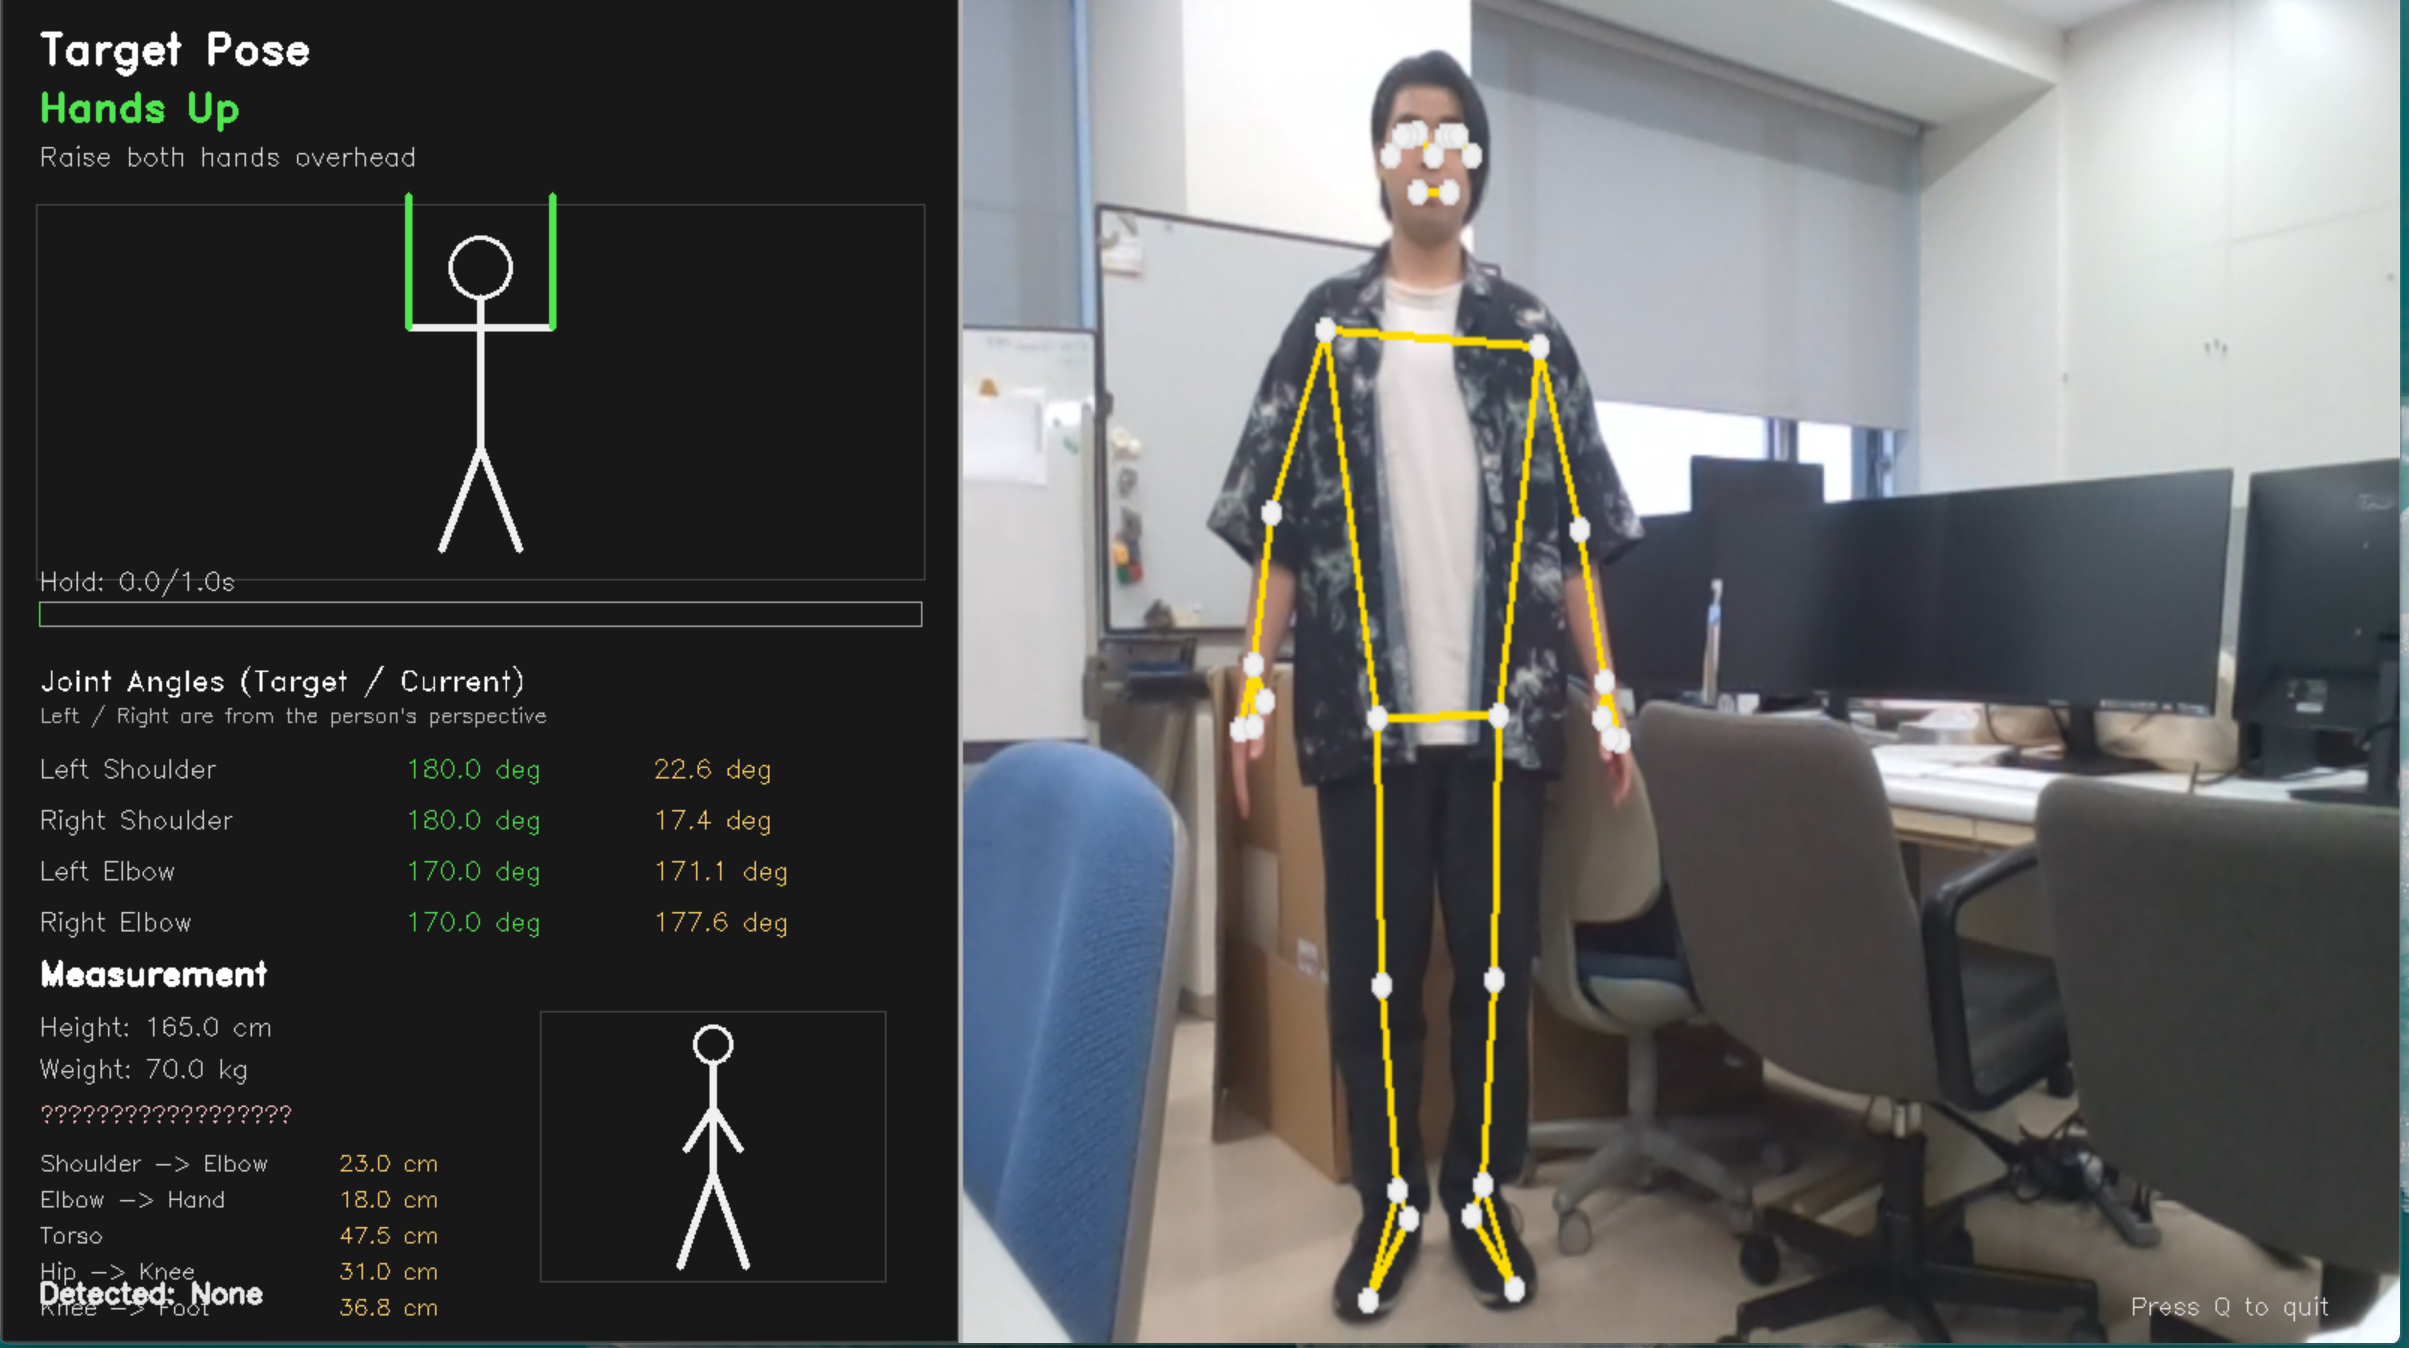
\includegraphics[clip,width=85mm,height=55mm]{motion_capture.pdf}
 \end{center}
 \vspace{-1.5em}
 \caption{MediaPipe使用例}
 \label{fig:MediaPipe}
 \vspace{-1.5em}
\end{figure}

\section{やること}
本研究では，カメラ映像から人体の骨格情報を取得し，目的に合わせたフォームへ修正するためのフィードバックをするシステムを構築する．

フォームの判定は，スクワットを構成する要素ごとに行う．
各要素に対応する関節の位置，関節間の長さおよびその比率，関節の角度といった情報が必要となる．
下半身全体の関節に加え，体幹の関節の座標を取得することで関節の位置，関節間の長さおよびその比率を取得することができる．
また直立状態の各関節の座標を基準として関節の角度を算出することで，関節の角度を取得することができる．
関節座標の取得は，オープンソースの機械学習フレームワークである MediaPipe を用いて，カメラ映像から人体の関節座標をリアルタイムに取得する．
MediaPipeからは\ref{fig:MediaPipe}のように手，手首，肘，肩，股関節，膝，足首，足の関節の座標を取得できる．
今回はスクワット動作に必要な関節座標を取得するため，肩，股関節，膝，足首，足の座標を使用する．

スクワットの各要素が利用者の目的に適しているか判定するシステムを構築する．
判定にあたっては，スクワット動作中の下肢の運動学的特徴に関する先行研究\cite{squat}を参考に，各目的に適したフォームを各要素ごとに定める．

\section{今後の予定}
各目的に適したフォームを各要素ごとに定め，スクワット動作中の関節座標を取得するシステムを構築する．

%\pagebreak
\begin{thebibliography}{99}
\bibitem{senior} 生き活きライフ(フレイル対策)部会: ``＜シニアの運動に関する意識調査＞毎日運動していても9割以上が筋力の低下を実感``, 2026/7/8参照
\url{https://prtimes.jp/main/html/rd/p/000000001.000146886.html}．

\bibitem{squat} Straub RK,Powers CM: ``A Biomechanical Review of the Squat Exercise: Implications for Clinical Practice.'', International Journal of Sports Physical Therapy. 2024;19(4):490-501．2026/7/15参照
\url{https://doi.org/10.26603/001c.94600}．

\bibitem{foam} Sigrist R,Rauter G,Riener R,Wolf P: ``Augmented visual, auditory, haptic, and multimodal feedback in motor learning: A review.'',Psychonomic Bulletin \& Review. 2013;20(1):21-53．2026/6/8参照
\url{https://link.springer.com/article/10.3758/s13423-012-0333-8}．



\end{thebibliography}
 
\end{document}
